\documentclass[10pt]{article}
\usepackage{tikz}
\pagestyle{empty}

\begin{document}

\vspace*{\fill}
\begin{center}
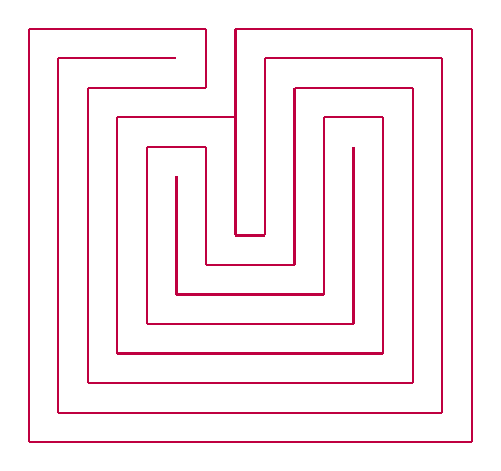
\begin{tikzpicture}[scale = 1.5, x = 0.25cm, y = -0.25cm, thick, purple]
% Horizontal lines
\draw(0, 0) -- (6, 0);
\draw(0, 14) -- (15, 14);
\draw(1, 1) -- (5, 1);
\draw(1, 13) -- (14, 13);
\draw(2, 2) -- (6, 2);
\draw(2, 12) -- (13, 12);
\draw(3, 3) -- (7, 3);
\draw(3, 11) -- (12, 11);
\draw(4, 4) -- (6, 4);
\draw(4, 10) -- (11, 10);
\draw(5, 9) -- (10, 9);
\draw(6, 8) -- (9, 8);
\draw(7, 0) -- (15, 0);
\draw(7, 7) -- (8, 7);
\draw(8, 1) -- (14, 1);
\draw(9, 2) -- (13, 2);
\draw(10, 3) -- (12, 3);
% Vertical lines
\draw(0, 0) -- (0, 14);
\draw(1, 1) -- (1, 13);
\draw(2, 2) -- (2, 12);
\draw(3, 3) -- (3, 11);
\draw(4, 4) -- (4, 10);
\draw(5, 5) -- (5, 9);
\draw(6, 0) -- (6, 2);
\draw(6, 4) -- (6, 8);
\draw(7, 0) -- (7, 7);
\draw(8, 1) -- (8, 7);
\draw(9, 2) -- (9, 8);
\draw(10, 3) -- (10, 9);
\draw(11, 4) -- (11, 10);
\draw(12, 3) -- (12, 11);
\draw(13, 2) -- (13, 12);
\draw(14, 1) -- (14, 13);
\draw(15, 0) -- (15, 14);
\end{tikzpicture}
\end{center}
\vspace*{\fill}

\end{document}
